\clearpage\subsection{Vertical Asymptotes}
Vertical asymptotes come about because of domain restrictions. Not all domain restrictions result in vertical asymptotes, but \textbf{all vertical asymptotes are a result of a domain restriction}. For example, the function $g(x) = \dfrac{1}{x}$ has a vertical asymptote at $x = 0$ because the function $g(x)$ has $x = 0$ excluded from its domain.

Because of this fact, we can find vertical asymptotes by solving for the domain restriction of a function and observing/determining its behavior as the function approaches the restriction. That is the process we used when first defining an asymptote in the previous section (plugging numbers closer and closer to $0$ and seeing what happens).

Let's try this on a practice problem.
\begin{problem}
    For the function, $f$, defined below, find it's vertical asymptotes.
    \[
        f(x) = \frac{1}{(x - 1)(x + 3)}
    \]
\end{problem}
This problem can be a little tricky, but you can solve it by remembering how to find the domain restriction of a function (dicussed in the earlier section). Read ahead to the solution when you're done or get stuck.

\begin{solution}
    To find the domain restriction of a function, we need to see if there's anything that could potentially "break" the function. In this case, we see that we have a fraction. That means we can break the function by making the denominator equal to $0$. To see what values of $x$ make the denominator equal to $0$, we can set it equal to $0$ and solve for $x$.
    \[
        (x - 1)(x + 3) = 0
    \]\clearpage
    Using the \textbf{Zero Product Property} (ZPP), we can see that this quadratic evaluates to $x = -3, 1$. Thus, $x = -3, 1$ are restricted from our domain. Now, we can see what happens to the function when we plug numbers extremely close to our domain restrictions.
    \[
    \begin{aligned}
        f(-3.0000001) &\approx 2499999.938\\
        f(-2.9999999) &\approx -2500000.063\\
        f(0.99999999) &\approx -25000000.06\\
        f(1.00000001) &\approx 24999999.94
    \end{aligned}
    \]
    We can see that plugging numbers close to our domain restrictions result in enormous numbers. This means that our asymptotes must be the lines $x = -3$ and $x = 1$.

    \begin{center}
        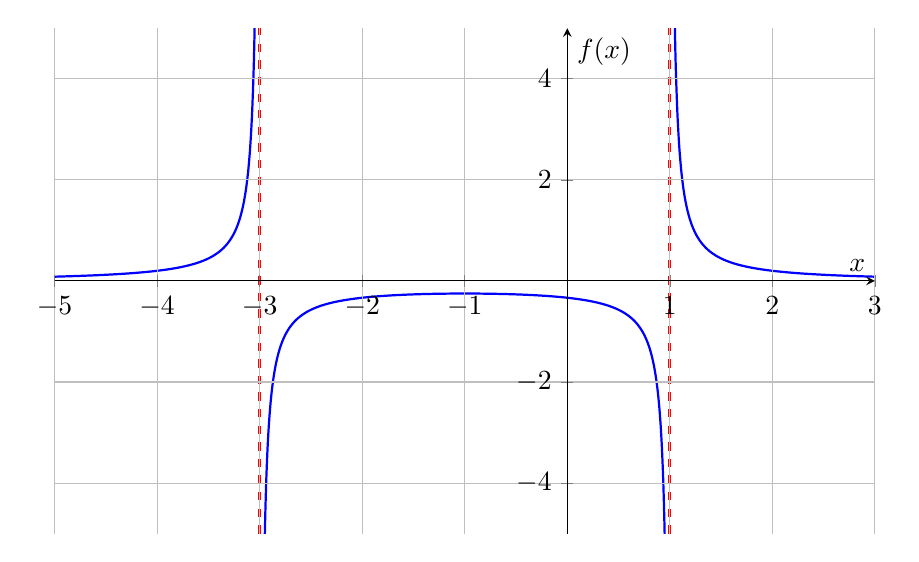
\begin{tikzpicture}
            \begin{axis}[
                axis lines = middle,
                xlabel = $x$, ylabel = {$f(x)$},
                xmin = -5, xmax = 3,
                ymin = -5, ymax = 5,
                grid = both,
                width = 12cm,
                height = 8cm,
                samples = 10,
                smooth,
                axis on top,
            ]
            \addplot[blue, thick, domain=-5:-3.01, samples=100] {1/((x-1)*(x+3))};
            \addplot[blue, thick, domain=-2.99:0.99, samples=300] {1/((x-1)*(x+3))};
            \addplot[blue, thick, domain=1.01:3, samples=100] {1/((x-1)*(x+3))};
            
            \draw[dashed, red, very thick] (axis cs:-3,\pgfkeysvalueof{/pgfplots/ymin}) -- (axis cs:-3,\pgfkeysvalueof{/pgfplots/ymax});
            \draw[dashed, red, very thick] (axis cs:1,\pgfkeysvalueof{/pgfplots/ymin}) -- (axis cs:1,\pgfkeysvalueof{/pgfplots/ymax});
            \end{axis}
        \end{tikzpicture}
    \end{center}
    
\end{solution}

\begin{problem}
    For the function, $g$, define below, find it's vertical asymptotes.
    \[
        g(x) = \frac{3}{x^2 + 1}
    \]
\end{problem}
Give it a shot. When you're done or get stuck, read ahead to the solution.
\begin{solution}
    Just like before, we can see that the denominator cannot equal $0$. So we can set it to $0$ and solve.
    \[
    x^2 + 1 = 0
    \]
    However, there's something different about this solution. If we let $a = 1$, $b = 0$, and $c = 1$, we can see that the discriminant ($b^2 - 4ac$) is less than $0$.
    \[
        0 - 4(1)(1) = -4
    \]
    This means that there are no real solutions to this quadratic. When the denominator set equal to $0$ has no real solutions, it means the function has no vertical asymptotes.

    \begin{center}
        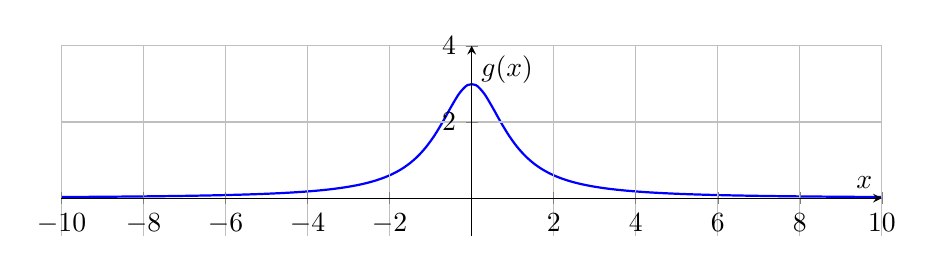
\begin{tikzpicture}
            \begin{axis}[
                axis lines = middle,
                xlabel = $x$, ylabel = {$g(x)$},
                xmin = -10, xmax = 10,
                ymin = -1, ymax = 4,
                grid = both,
                width = 12cm,
                height = 4cm,
                samples = 10,
                smooth,
                axis on top,
            ]
            \addplot[blue, thick, domain=-10:10, samples=100] {3/(x^2 + 1)};
            \end{axis}
        \end{tikzpicture}
    \end{center}
\end{solution}